\documentclass[twocolumn]{article}
\usepackage[utf8]{inputenc}
\usepackage{graphicx}
\usepackage{amsmath}
\usepackage{booktabs}
\usepackage{geometry}
\geometry{a4paper, margin=0.75in}

\title{Machine Learning for Survival Prediction in Heart Failure Patients: A Clinical Factor Analysis}
\author{Haoyu Wang}
\date{March 2026}

\begin{document}

\maketitle

\begin{abstract}
Predicting the survival of heart failure patients is critical for clinical intervention. This study utilizes a Multi-Layer Perceptron (MLP) model to analyze clinical records. Our results demonstrate that time, serum creatinine, and ejection fraction are the most significant predictors, with the model achieving an accuracy of 0.70.
\end{abstract}

\section{Introduction}
Heart failure remains a leading cause of mortality worldwide. Artificial Intelligence provides a robust framework for risk stratification. This paper evaluates the effectiveness of deep learning models in prognostic assessments.

\section{Methods}
We implemented a Multi-Layer Perceptron (MLP) using Python and Scikit-learn. Data was standardized using Z-score normalization to ensure model stability. Figure \ref{fig:workflow} illustrates our AI-driven diagnostic workflow.

\begin{figure}[htbp]
    \centering
    % 注意：请确保你在 Overleaf 上传的 AI 概念图片文件名叫 ai_workflow.jpg
    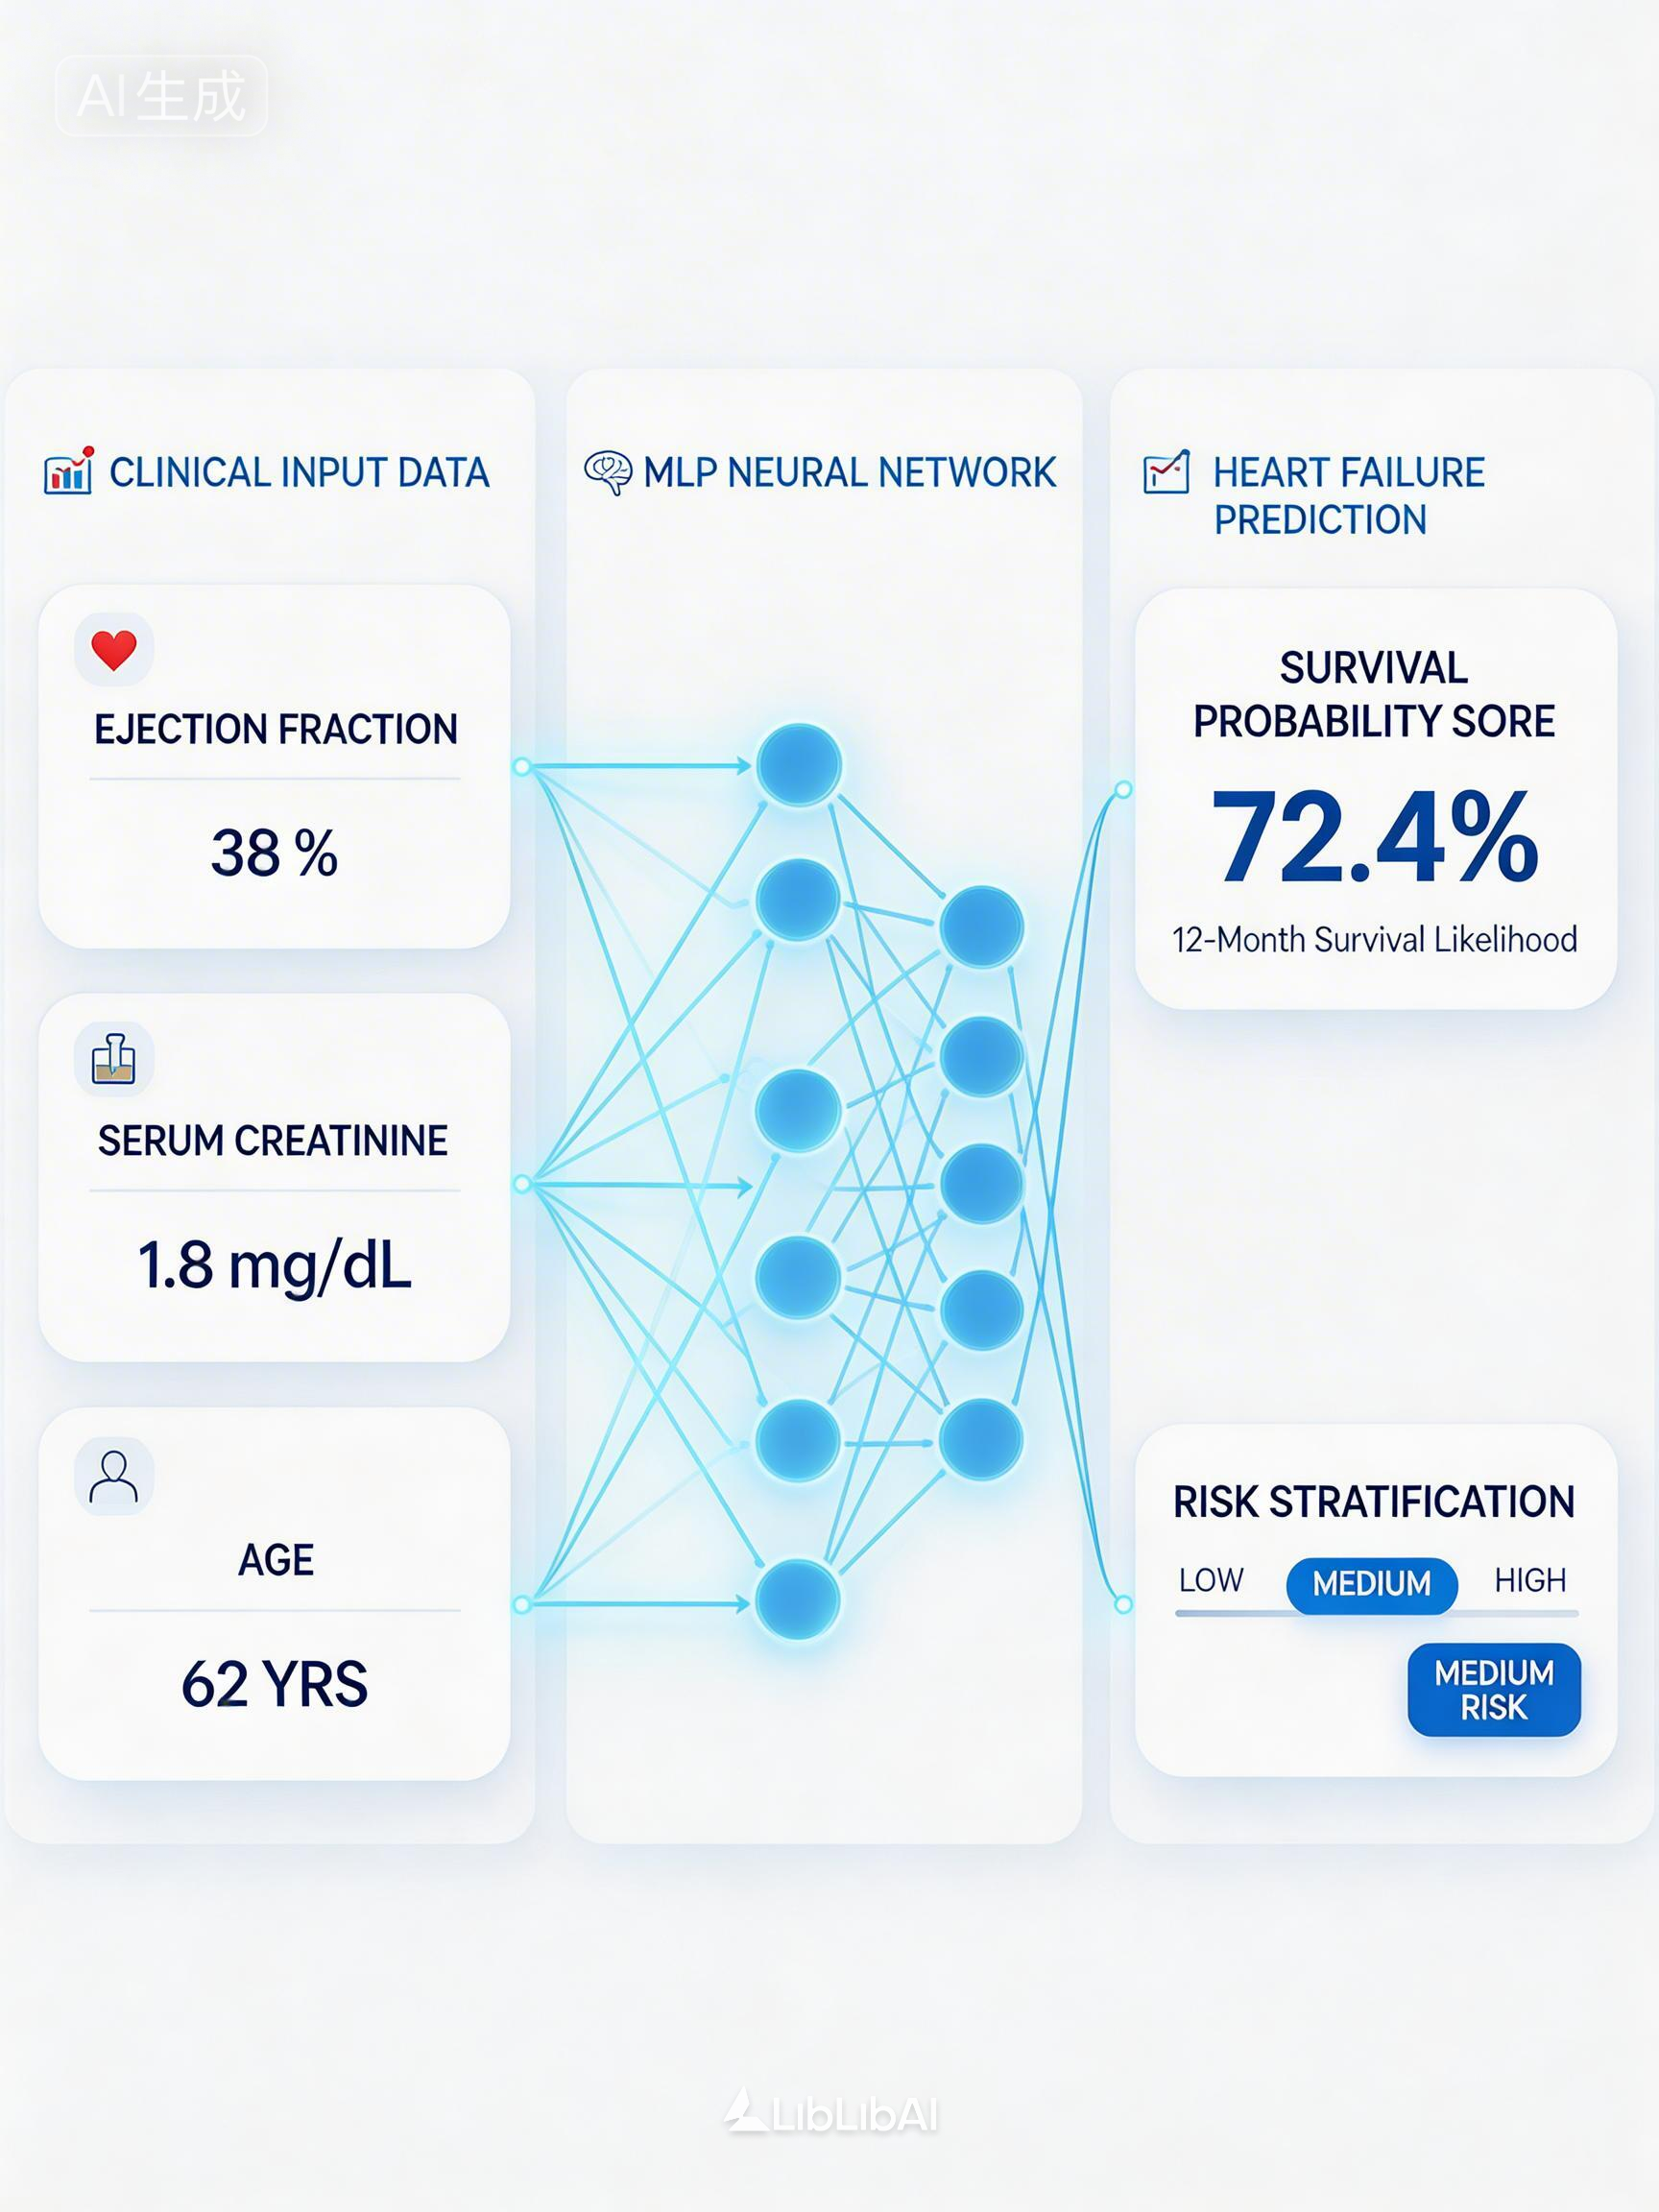
\includegraphics[width=0.45\textwidth]{ai_workflow.jpg}
    \caption{Conceptual AI workflow for heart failure prediction.}
    \label{fig:workflow}
\end{figure}

\section{Results}
The feature importance analysis (Fig. \ref{fig:heatmap}) identified three primary risk factors: follow-up time (37.5\%), serum creatinine (15.5\%), and ejection fraction (11.2\%). 

\begin{figure}[htbp]
    \centering
    % 注意：请确保你在 Overleaf 上传的热力图片文件名叫 correlation_heatmap.png
    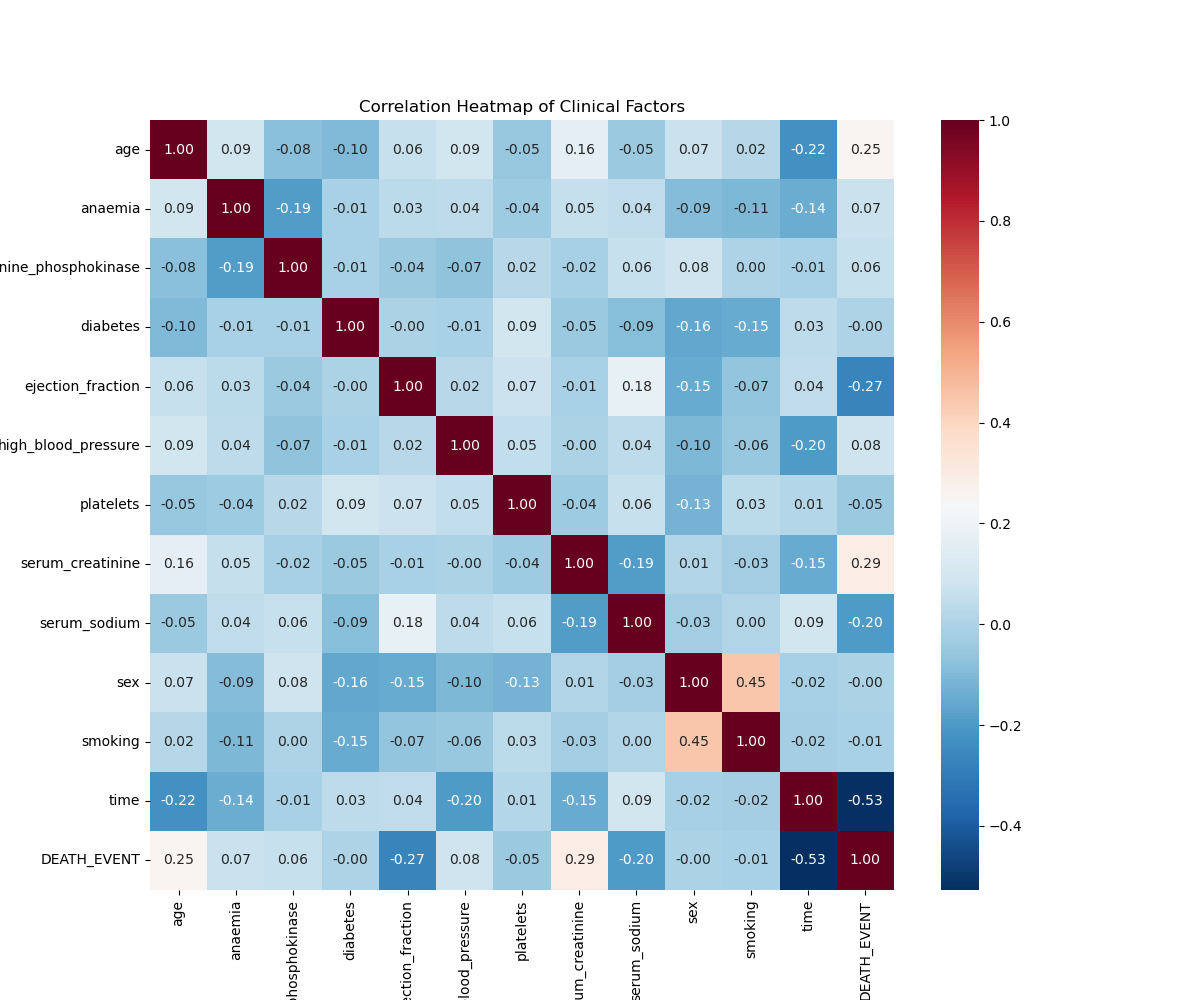
\includegraphics[width=0.45\textwidth]{correlation_heatmap.png}
    \caption{Correlation heatmap of clinical features.}
    \label{fig:heatmap}
\end{figure}

The MLP model's performance was evaluated using the $F_1$ score, calculated as:
\begin{equation}
F_1 = 2 \cdot \frac{\text{precision} \cdot \text{recall}}{\text{precision} + \text{recall}}
\end{equation}
Our model achieved a weighted $F_1$ score of 0.69 and an accuracy of 0.70.

\section{Discussion}
Serum creatinine levels directly reflect renal perfusion, which is often compromised in advanced heart failure (Cardiorenal Syndrome). The high importance of follow-up time suggests the necessity of continuous monitoring.

\section{Conclusion}
AI models can effectively assist clinicians in prognostic assessments, providing a scientific basis for personalized treatment plans.

\end{document}
